\chapter{理論}
\begin{comment}
\section{イオントラップ}
電荷を持つイオンは電場によって力を受けることから,電磁場を用いることで空間に閉じ込めることが可能になっている.これを可能にする装置をイオントラップと呼ぶ.電磁気学において,アーンショーの定理と呼ばれる定理が知られており,この定理によれば静電ポテンシャルを記述するラプラス方程式の解に極大値および極小値が表れない.つまり,静電場のみを用いてイオンを捕獲することが不可能になっている.イオンを閉じ込めるためには,静電場と静磁場を使ったペニンブトラップ,あるいはrf(radio frequency)電場と静電場を用いたパウルトラップが主に使用される.本研究では後者のパウルトラップの原理を応用させた平面型のイオントラップ.プレーナートラップを使用してイオンの捕獲を行っていることから,パウルトラップについて述べる.
\section{パウルトラップ}
\subsection{rf擬ポテンシャル}
\large
\begin{align}
	\Phi_{\rm eff}(x,y,z) = \frac{e}{4m\Omega_{\rm rf}}|\vec{E}(x,y,z)|^2
\end{align}
\normalsize


\subsection{イオンの運動}
Mathieu方程式
\large
\begin{align}
	\frac{{\rm d^2}r_i}{{\rm d}t^2} + [a_\alpha + 2q_\alpha \cos (\Omega_{\rm rf} t)]\frac{\Omega_{\rm rf}^2}{4}r_i = 0. \quad (i = x,y,z)
\end{align}
\normalsize
\subsection{余剰マイクロ運動}
浮遊電場が存在する場合のMathieu方程式
\large
\begin{align}
	\frac{{\rm d^2}r_i}{{\rm d}t^2} + [a_i + 2q_i \cos (\Omega_{\rm rf} t)]\frac{\Omega_{\rm rf}^2}{4}r_i = \frac{e\vec{E}_{\rm stray}\cdot \hat{r}_i}{m}. \quad (i = x,y,z)
\end{align}
\normalsize
rfに起因,レーザーによって冷却することができない
\clearpage
\section{プレーナートラップ}
\begin{figure}[h]
	\begin{center}
		\begin{minipage}{0.48\linewidth}
			\begin{center}
			\includegraphics[width = 0.98\columnwidth]{./theory/figure/PaulTrap_3Dto2D_3DTrap.png}
			\end{center}
		\end{minipage}
		\begin{minipage}{0.48\linewidth}
			\begin{center}
			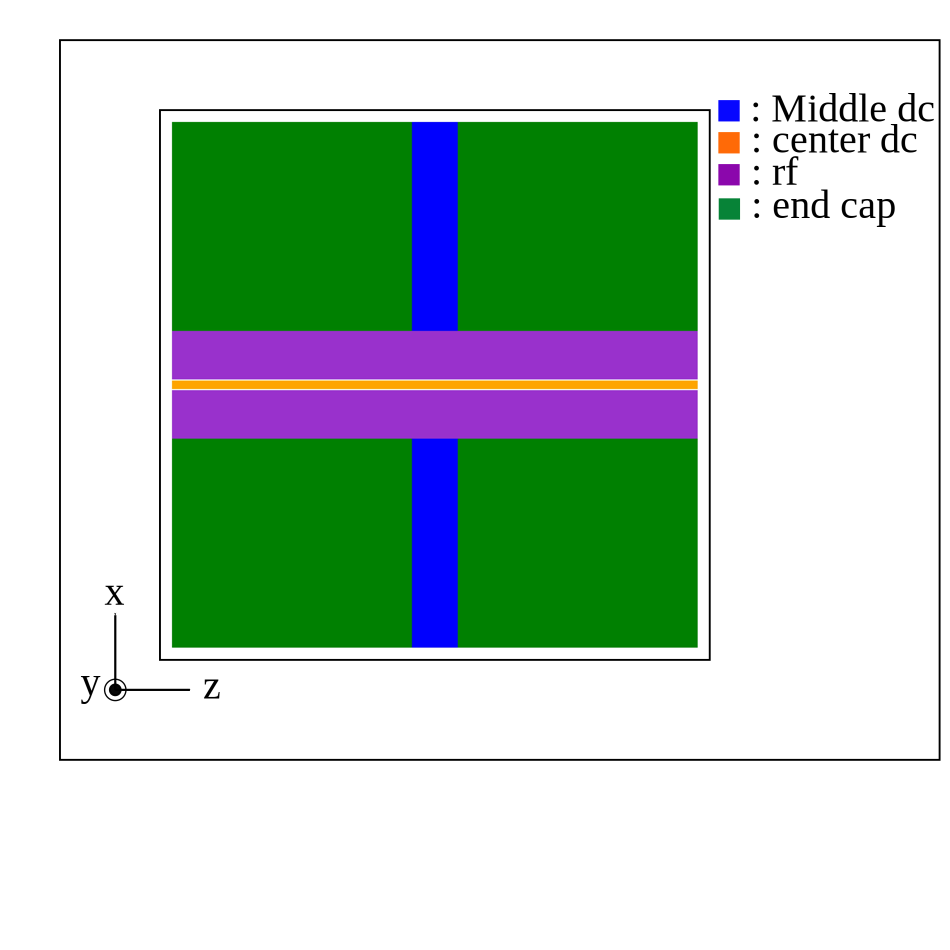
\includegraphics[width = 0.98\columnwidth]{./theory/figure/PaulTrap_3Dto2D_2DTrap.png}
			\end{center}
		\end{minipage}
	\end{center}
	\caption{a}
\end{figure}
\subsection{電極の仕様}
\begin{figure}[h]
	\begin{center}
		\includegraphics[width = 0.5\linewidth]{./theory/figure/named_electrode.png}
		\caption{本実験で使用するプレーナートラップの電極モデル}
		\label{fig:Named_PlannerTrap}
	\end{center}
\end{figure}
\subsection{矩形電極が作る静電ポテンシャル}
\begin{figure}[h]
	\begin{center}
		\includegraphics[width = 0.5\linewidth]{./theory/figure/Potential_of_rect-electrode.png}
		\caption{$(z_1,x_1),(z_2,x_2)$で指定される矩形が任意の点$(x,y,z)$に形成する静電ポテンシャル}
		\label{fig:Potential_from_rect-electrode}
	\end{center}
\end{figure}
\begin{align}\label{eq:rectangle_electrode}
	\phi(x,y,z) = \frac{V}{2\pi} \left\lbrace \arctan \left[ \frac{(x_2 - x)(z_2 - z)}{y\sqrt{y^2 + (x_2 - x)^2 + (z_2 - z)^2}}\right] - \arctan \left[ \frac{(x_1 - x)(z_2 - z)}{y\sqrt{y^2 + (x_1 - x)^2 + (z_2 - z)^2}} \right]  \right.  \notag \\ 
	\left. -\arctan \left[ \frac{(x_2 - x)(z_1 - z)}{y\sqrt{y^2 + (x_2 - x)^2 + (z_1 - z)^2}}\right] + \arctan \left[ \frac{(x_1 - x)(z_1 - z)}{y\sqrt{y^2 + (x_1 - x)^2 + (z_1 - z)^2}} \right]  \right\rbrace 
\end{align}
\section{レーザー冷却}

\end{comment}

\section{画像処理によるイオン捕獲位置と電場の算出}
OpenCVとNumpyを使って画像処理を行うことでイオンの位置と,イオンの位置における電場の算出を行う.ここでは画像処理の方法について述べる.
\subsection{ヒストグラムの正規化}
カメラでイオンの蛍光を撮像する際に,カメラの集光時間やピントおよび照射するレーザーの波長や位置などによって得られるイオン捕獲画像の輝度値のヒストグラムは変化する.輝度値が0に近い画素が多ければ画像は全体として暗く,255に近い画素が多ければ画像は全体として明るくなる.\Fig{ionimage}に示すイオン捕獲画像を例にヒストグラムの偏りを\Fig{hist}に示す.
\begin{figure}[h]
	\begin{center}
	\begin{minipage}{0.3\linewidth}
		\includegraphics[width=0.98\columnwidth]{./theory/figure/5/image_0.jpg}
	\end{minipage}
	\begin{minipage}{0.3\linewidth}
		\includegraphics[width=0.98\columnwidth]{./theory/figure/5/image_2.jpg}
	\end{minipage}
	\begin{minipage}{0.3\linewidth}
		\includegraphics[width=0.98\columnwidth]{./theory/figure/5/image_1.jpg}
	\end{minipage}
	\end{center}
	\caption{集光系のピントおよびレーザー照射位置などが異なる場合のイオン捕獲画像}
	\label{fig:ionimage}
\end{figure}

\begin{figure}[h]
	\begin{center}
		\begin{minipage}{0.3\linewidth}
			\includegraphics[width=0.98\columnwidth]{./theory/figure/5/hist_0.jpg}
		\end{minipage}
		\begin{minipage}{0.3\linewidth}
			\includegraphics[width=0.98\columnwidth]{./theory/figure/5/hist_2.jpg}
		\end{minipage}
		\begin{minipage}{0.3\linewidth}
			\includegraphics[width=0.98\columnwidth]{./theory/figure/5/hist_1.jpg}
		\end{minipage}
	\end{center}
	\caption{\Fig{ionimage}の各画像のピクセル輝度値のヒストグラム}
	\label{fig:hist}
\end{figure}

イオンの位置特定を行うに際し,二値化の処理のための閾値を定める.しかし,\Fig{hist}のように輝度値の偏りが各画像において異なっている場合,閾値を画像毎に変化させる必要がある.これを防ぐために濃度諧調変換と呼ばれるヒストグラムの正規化を行う.[c,d]の画素値を持つ画像を[a,b]のレンジに変換する式は次式で与えられる.

\large
\begin{align}\label{eq:GS_trans}
x_{\rm out} = 
\left\{ 
\begin{array}{ll}
	a & {\rm if} \ x_{\rm in} < c \\
	\frac{b-a}{d-c}(x_{\rm in}-c) + a & {\rm else \ if} \ c \leq x_{\rm in} < d \\
	b &{\rm else}
\end{array} \right.
\end{align}
\normalsize

\Fig{hist}に対して\Eq{GS_trans}を$a=0,b=255$として適用させると\Fig{hist_norm}となる.
\begin{figure}[h]
	\begin{center}
		\begin{minipage}{0.3\linewidth}
			\includegraphics[width=0.98\columnwidth]{./theory/figure/5/norm_hist_0.jpg}
		\end{minipage}
		\begin{minipage}{0.3\linewidth}
			\includegraphics[width=0.98\columnwidth]{./theory/figure/5/norm_hist_2.jpg}
		\end{minipage}
		\begin{minipage}{0.3\linewidth}
			\includegraphics[width=0.98\columnwidth]{./theory/figure/5/norm_hist_1.jpg}
		\end{minipage}
	\end{center}
	\caption{\Fig{ionimage}の各画像のピクセル輝度値のヒストグラムを正規化したもの}
	\label{fig:hist_norm}
\end{figure}



\subsection{イオンの検出および,捕獲位置と電場の算出方法}